\documentclass{article}

% if you need to pass options to natbib, use, e.g.:
% \PassOptionsToPackage{numbers, compress}{natbib}
% before loading nips_2018

% ready for submission
% \usepackage{nips_2018}

% to compile a preprint version, e.g., for submission to arXiv, add
% add the [preprint] option:
% \usepackage[preprint]{nips_2018}

% to compile a camera-ready version, add the [final] option, e.g.:
\usepackage[final]{nips_2018}

% to avoid loading the natbib package, add option nonatbib:
% \usepackage[nonatbib]{nips_2018}

\usepackage[utf8]{inputenc} % allow utf-8 input
\usepackage[T1]{fontenc}    % use 8-bit T1 fonts
\usepackage{hyperref}       % hyperlinks
\usepackage{url}            % simple URL typesetting
\usepackage{booktabs}       % professional-quality tables
\usepackage{amsfonts}       % blackboard math symbols
\usepackage{nicefrac}       % compact symbols for 1/2, etc.
\usepackage{microtype}      % microtypography
\usepackage{subcaption}
\usepackage{graphicx}
\usepackage{bbm}
\usepackage{amsmath}

\title{Deep Learning 2018 - Assignment 1}

% The \author macro works with any number of authors. There are two
% commands used to separate the names and addresses of multiple
% authors: \And and \AND.
%
% Using \And between authors leaves it to LaTeX to determine where to
% break the lines. Using \AND forces a line break at that point. So,
% if LaTeX puts 3 of 4 authors names on the first line, and the last
% on the second line, try using \AND instead of \And before the third
% author name.

\author{
  David Rau (11725184) \\ 
  University of Amsterdam \\
  \texttt{david.rau@student.uva.nl} \\
  %% examples of more authors
  %% \And
  %% Coauthor \\
  %% Affiliation \\
  %% Address \\
  %% \texttt{email} \\
  %% \AND
  %% Coauthor \\
  %% Affiliation \\
  %% Address \\
  %% \texttt{email} \\
  %% \And
  %% Coauthor \\
  %% Affiliation \\
  %% Address \\
  %% \texttt{email} \\
  %% \And
  %% Coauthor \\
  %% Affiliation \\
  %% Address \\
  %% \texttt{email} \\
}

\begin{document}
% \nipsfinalcopy is no longer used

\maketitle



\section{MLP backprop and NumPy implementation}


\subsection{Analytical derivation of gradients}

\subsubsection*{Question 1.1 a}
\begin{equation}
\frac{\partial L }{\partial x_i^{(N)}} = \frac{\partial - \log x^{(N)}_{\operatorname{argmax}_t}}{\partial x_i^{(N)}} = \frac{1}{x_i^{(N)}}\mathbbm{1}(i=\operatorname{argmax}_t)
\end{equation}

\begin{equation}
\begin{aligned}
\frac{\partial x_i^{(N)} }{\partial \tilde{x}_j^{(N)}} 
& = \frac{\partial \frac{\exp(\tilde{x}_i^{(N)})}{\sum_{k=1}^{d_N} \exp(\tilde{x}_k^{(N)}}}{\partial \tilde{x_j}^{(N)}} 
= \frac{\tilde{x_i}^{(N)} \sum_{k=1}^{d_N} \exp(\tilde{x}_k^{(N)}) -  \tilde{x_j}^{(N)} \tilde{x_i}^{(N)}}{\Big(\sum_{k=1}^{d_N} \exp(\tilde{x}_k^{(N)}) \Big)^2} \\
 \\
& = \frac{\tilde{x_i}^{(N)}}{\sum_{k=1}^{d_N} \exp(\tilde{x}_k^{(N)}} \Bigg(1 -\frac{\exp(\tilde{x}_j)^{(N)}}{\sum_{k=1}^{d_N} \exp(\tilde{x}_k^{(N)}} \Bigg) 
=\text{Softmax}(\tilde{x}_i^{(N)})\big( \mathbbm{1}(i=j) - \text{Softmax}(\tilde{x}_j^{(N)} \big) \\
\end{aligned}
\end{equation}

\begin{equation}
\frac{\partial x_i^{(l<N)} }{\partial \tilde{x}_j^{(l<N)}} = 
\frac{\partial \max(0, x_i^{(l)}) }{\partial \tilde{x}_j^{(l<N)}} = \mathbbm{1}(i=j)\mathbbm{1}(x_j^{(l)} > 0)
\end{equation}

\begin{equation}
\frac{\partial \tilde{x}_i^{(l)} }{\partial x_j^{(l-1)}} = 
\frac{\partial \sum_{k=1}^L W_{jk}^{(l)} x_i^{(l-1)} + b_i^{(l)} }{\partial x_j^{(l-1)}} =  \mathbbm{1}(i=j) W_{jk}^{(l)}
\end{equation}

\begin{equation}
\frac{\partial \tilde{x}_i^{(l)}}{\partial W_{jk}^{(l)}} = 
\frac{\partial \sum_{k=1}^L W_{ik}^{(l-1)} x_i^{(l)} + b_i^{(l-1)}}{\partial W_{jk}^{(l)}} = \mathbbm{1}(i=j) x_j^{(l)}
\end{equation}

\begin{equation}
\frac{\partial \tilde{x_i}^{(l)} }{\partial b_i^{(l)}} = 
\frac{\partial \sum_{k=1}^L W_{ik}^{(l-1)} x_i^{(l)} + b_i^{(l-1)}}{\partial b_j^{(l)}} = \mathbbm{1}(i=j)
\end{equation}

\subsubsection*{Question 1.1 b}
\begin{equation}
	\frac{\partial L}{\partial \tilde{x}^{(N)}} = \frac{\partial L}{\partial x^{(N)}} \frac{\partial x^{(N)}}{\tilde{x}^{(N)}} = \frac{\partial L}{\partial x^{(N)}} \mathbbm{1}_{N_D}x^{(N)} - x^{(N)}x^{(N)^T}
\end{equation}


\begin{equation}
	\frac{\partial L}{\partial \tilde{x}^{(l<N)}} = \frac{\partial L}{\partial x^{(l<N)}} \frac{\partial x^{(l<N)}}{\tilde{x}^{(l<N)}} = \frac{\partial L}{\partial x^{(l<N)}} \cdot \mathbbm{1} (x^{(l<N)} > 0)
\end{equation}

\begin{equation}
	\frac{\partial L}{\partial \tilde{x}^{(l<N)}} = \frac{\partial L}{\partial \tilde{x}^{(l+1)}}\frac{\partial \tilde{x}^{(l+1)}}{\partial x^{(l)}}
	= \frac{\partial L}{\partial \tilde{x}^{(l+1)}} W^{(l)^T}
\end{equation}



\begin{equation}
	\frac{\partial L}{\partial W^{(l)}} = \frac{\partial L}{\partial \tilde{x}^{(l)}}\frac{\partial \tilde{x}^{(l)}}{\partial W^{(l)}}
	= x^{(l)^T}\frac{\partial L}{\partial \tilde{x}^{(l)}} 
\end{equation}


\begin{equation}
	\frac{\partial L}{\partial b^{(l)}} = \frac{\partial L}{\partial \tilde{x}^{(l)}}\frac{\partial \tilde{x}^{(l)}}{\partial b^{(l)}}
	=\frac{\partial L}{\partial \tilde{x}^{(l)}} \mathbbm{1}_{d_l}
\end{equation}


\subsubsection*{Question 1.1 c}
The equations for batch size $\neq$ 1 remain mostly the same. However, as the derivative of the loss with respect to the previous layer is a matrix all derivatives have now to be taken with respect to the matrix. The loss of the Cross Entropy has now to be calculated with respect to the different batches $(s)$:
\begin{equation}
	\frac{\partial L_{\text{total}}}{\partial \tilde{x}^{(s,N)}} = \frac{\partial L_{\text{total}} }{L_{\text{individual}}^s} \frac{\partial L_{\text{individual}}^s }{\partial \tilde{x}^{(s, N)}}
\end{equation}

where

\begin{equation}
	\frac{\partial L_{\text{total}} }{L_{\text{individual}}^s} = \frac{1}{B}
\end{equation}

\subsection{NumPy implementation}
\subsubsection*{Question 1.2}

Since it wasn't explicitly stated which loss we were supposed to report I decided to show the batch loss and refer to in the following as 'loss'.
\bigskip

The accuracy and loss curves of the of the numpy implementation of the MLP can be found in Fig. \ref{numpy_mlp}. The model was trained with the default parameters. The top accuracy within the training was 47.25\%. As it can be seen of the bottom of Fig. \ref{numpy_mlp} the loss goes quickly down in the beginning and then stabilizes at around 1.5. The Accuracy curve of the whole validation set has a steep slope at the beginning and then saturates around 46\%.
\begin{figure*}[h!]
    \centering
  \centering
  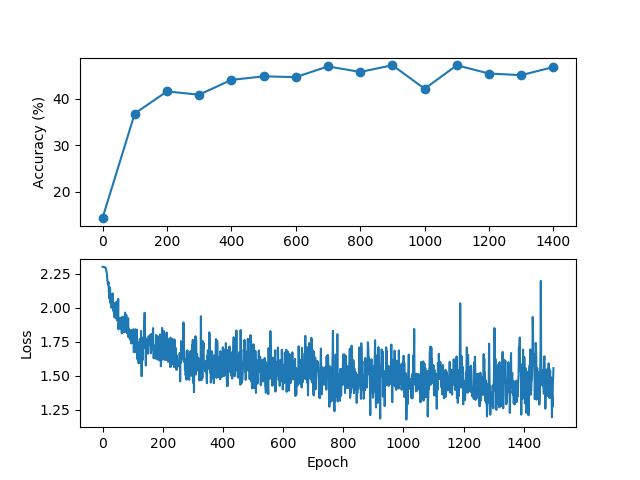
\includegraphics[scale=0.5]{numpy_mlp.png}
  \caption{Accuracy (in \%) and loss curves of the Numpy MLP for default values of parameters: batch size : 200, learning rate : 0.002 and dnn hidden units : 100. The top accuracy on the whole test set within the training was 47.24\%.}
  \label{numpy_mlp}
\end{figure*}



\section{PyTorch MLP}
\subsubsection*{Question 2}

First I ran the pytorch implementation with default configuration and reached 45.53\% accuracy on the test set after 1500 epochs. Then I increased the hidden layers to two hidden layers with 100 units respectively to increase the model complexity in order to cope with the high dimensional input. This achieved a accuracy of 43.39\% after 1500 epochs and 46.1\% after 3500 epochs. Two hidden layers of size 200 achieved  47.82\% after 3500 epochs and the accuracy stabilised around that value. In the following all models were therefore trained for 3500 epochs. \\
In order to cope with the problem that ReLUs die out in deeper networks I added a batch normalization layer before each linear layer. The accuracy went up to  54.03\%. Because Batch normalization layers allow for bigger learning rates i changed the learning rate from 0.002 to 0.02 and retrained. This however couldn't improve the performance. As a last experiment I added a dropout layer with probability 0.2 to every linear layer this also couldn't improve the accuracy further probably because the learning is already saturated. However, by adding l1 weight regularization for the linear layers I could achieve the highest accuracy of 56.06\%. The accuracy curve as well as the loss curve can be found in Fig. \ref{tuned_pytorch}.

\begin{figure*}[h!]
    \centering
  \centering
  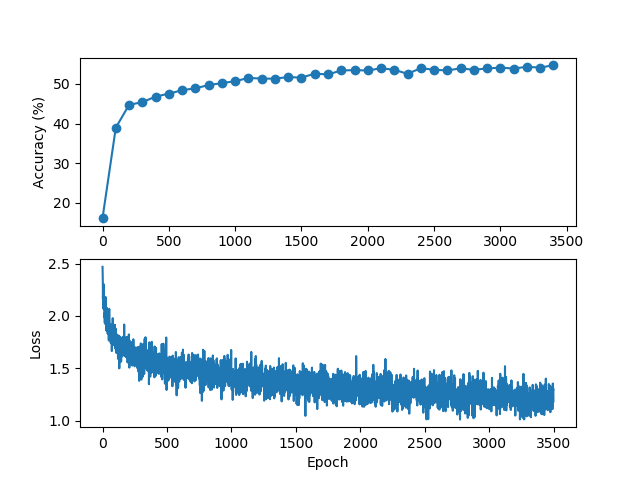
\includegraphics[scale=0.5]{_lr_0_02_l1_True_batch_norm_True_dropout_True_h_200,200.png}
  \caption{Accuracy (in \%) and loss curves of the Pytorch MLP for parameters: batch size : 200, learning rate : 0.02, batch normalization, l1 regularization, dropout 0.2, with two hidden layers of size 200. The top accuracy on the whole test set within the training is 56.06\%.}
  \label{tuned_pytorch}
\end{figure*}




\section{Custom Module: Batch Normalization}
\subsubsection*{Question 3.2 a}
\begin{equation}	
	\Big(\frac{\partial L}{\partial \gamma}\Big)_j = \sum_s \sum_i \frac{\partial L}{\partial y_i^s} \frac{\partial y_i^s}{\partial \gamma_j} = \sum_s \sum_i \frac{\partial L}{\partial y_i^s} \frac{\partial \gamma_i \hat{x}_i^s + \beta_i}{\partial \gamma_j} = \sum_s \frac{\partial L}{\partial y_i^s} \mathbbm{1}(i=j) \hat{x}_j^s
\end{equation}
\begin{equation}
	\Big(\frac{\partial L}{\partial \beta}\Big)_j = \sum_s \sum_i \frac{\partial L}{\partial y_i^s} \frac{\partial y_i^s}{\partial \beta_j} = \sum_s \sum_i \frac{\partial L}{\partial y_i^s} \frac{\partial \gamma_i \hat{x}_i^s + \beta_i}{\partial \beta_j} = \sum_s \frac{\partial L}{\partial y_i^s} \mathbbm{1}(i=j) 1
\end{equation}


\begin{equation}
	\Big(\frac{\partial L}{\partial x}\Big)_j^r = \sum_s \sum_i \frac{\partial L}{\partial y_i^s} \frac{\partial y_i^s}{\partial x_j^r} = 
\end{equation}



\section{PyTorch CNN}

\subsubsection*{Question 4}
As the top accuracy (78\%) on the validation set of the CNN in Fig. \ref{convnet} suggests, CNNs are the appropriate network architecture to tackle this task. The CNN was trained with the default parameters: batch size 32 and learning rate 0.0001. As it can be seen in Fig. \ref{convnet} the batch loss stabilises below 1. Moreover, it could be interesting to examine the validation loss. If the validation loss would up while the batch loss goes still down the network is overfitting.
\begin{figure*}[h!]
    \centering
  \centering
  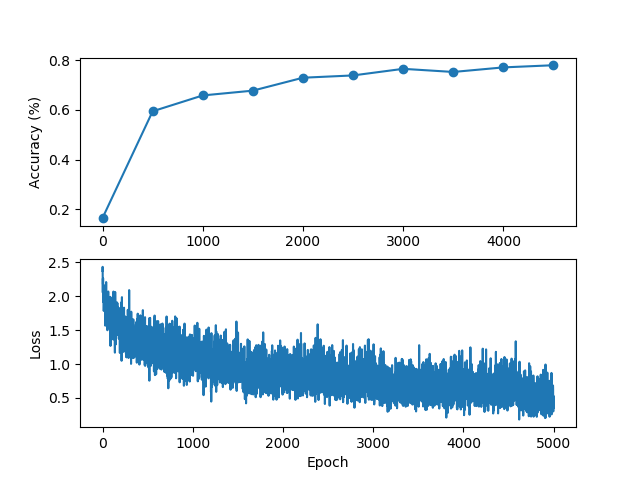
\includegraphics[scale=0.5]{convnet.png}
  \caption{Accuracy (in \%) and loss curves of the Pytorch ConvNet for default values of parameters: batch size : 32, learning rate : 0.0001. The top accuracy on the whole test set within the training is 78\%.}
  \label{convnet}
\end{figure*}


\end{document}
